\documentclass{beamer}

% Preámbulo - Parte A

\usepackage[utf8]{inputenc} % Soporte para los acentos
\usepackage[T1]{fontenc}

\usepackage{xcolor} % Usar colores
\usepackage{pstricks}

% Paquetes adicionales de símbolos matemáticos
\usepackage{amsmath,amssymb,amsfonts,latexsym,cancel} 

\usepackage{booktabs} % Opciones adicionales para el entorno tabular
\usepackage{longtable} % Para tablas de más de una página

\usepackage{multirow}

\DeclareGraphicsExtensions{.pdf,.png,.jpg}
\usefonttheme{professionalfonts}
\usetheme{Warsaw}
\setbeamercovered{transparent}

\section{Procesamiento Digital de Señales}

\begin{document}

\title{Verificación de Hablantes a través de la Voz}
\subtitle{Trabajo Final de Procesamiento Digital de Señales}
\author{Iván F. Schweikofski,
        Camila Saucedo y 
        Darién J. Ramírez \\ Tutor: Matias F. Gerard}
\date{\empty}

\frame{\titlepage}

% 1
\begin{frame}{Introducción} %\frametitle{} \framesubtitle{}

\centering\fbox{Identificación automática del hablante}

\begin{columns}[t]
\begin{column}{0.5\linewidth}
\begin{block}{Identificación del hablante}
Decidir si la persona está o no dentro de un conjunto de personas.
\end{block}
\end{column}

\begin{column}{0.5\linewidth}
\begin{block}{Verificación del hablante}
Decidir si el hablante es quien dice ser.
\end{block}
\end{column}
\end{columns}

\end{frame}

% 2
\begin{frame}{Implementación}

\begin{columns}
\begin{column}{0.5\linewidth}
\begin{enumerate}
\item Base de datos.
\item Señal de entrada.
\item Ventaneo de la señal de entrada.
\item Selección de ventanas sonoras.
\item Extracción de características ($F_{0}$, Formantes y MFCC).
\item Comparación mediante DTW.
\item Decisión.
\end{enumerate}
\end{column}

\begin{column}{0.5\linewidth}
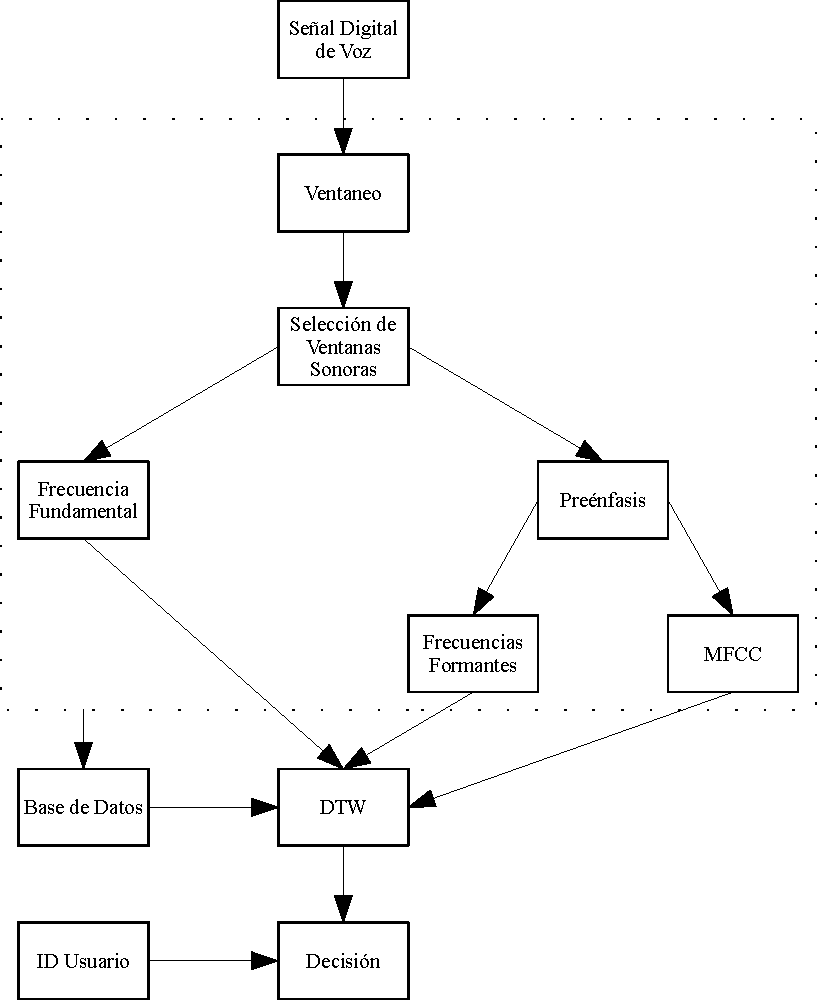
\includegraphics[width=\linewidth]{23}
\end{column}

\end{columns}

\end{frame}

% 3
\begin{frame}{Sonidos sonoros y sonidos sordos}

\begin{columns}
\begin{column}{0.6\linewidth}
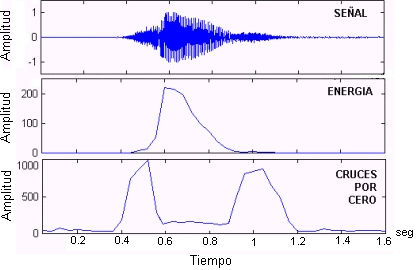
\includegraphics[width=\linewidth]{sonoro}
\end{column}

\begin{column}{0.4\linewidth}

\begin{block}{}
Ventaneo con ventanas sonoras.
\end{block}

\begin{enumerate}
\item \textit{Sonidos sonoros:} baja cantidad de cruces por cero y alta energía. Periodicidad.
\item \textit{Sonidos sordos:} mayor densidad de cruces por cero y menor energía.
\end{enumerate}
\end{column}
\end{columns}

\end{frame}

% 4
\begin{frame}{Frecuencia fundamental $F_{0}$}

\begin{enumerate}
\item Autocorrelación.
\item $\displaystyle \frac{1}{f_{}max}=
\frac{1}{300} \leq T_{0} \leq \frac{1}{50}=\frac{1}{f_{min}}$
\end{enumerate}

\begin{center}
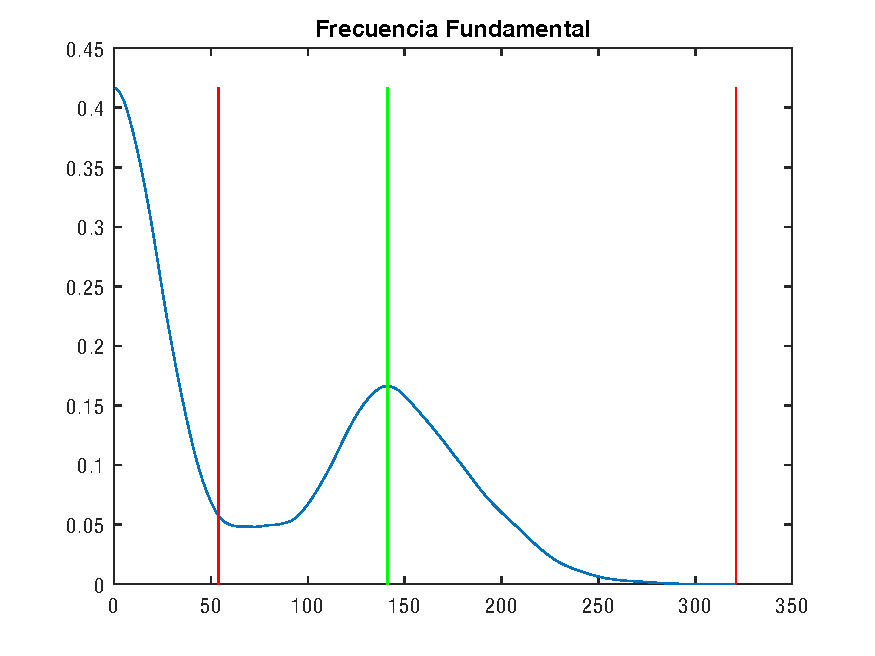
\includegraphics[scale=0.5]{F0}
\end{center}

\end{frame}

%
\begin{frame}{Preénfasis}

\begin{align*}
y[n] &= x[n]-ax[n-1] & 0.9\leq a\leq 0.97 && y[1] &= x[1]
\end{align*}

\begin{columns}
\begin{column}{0.5\linewidth}
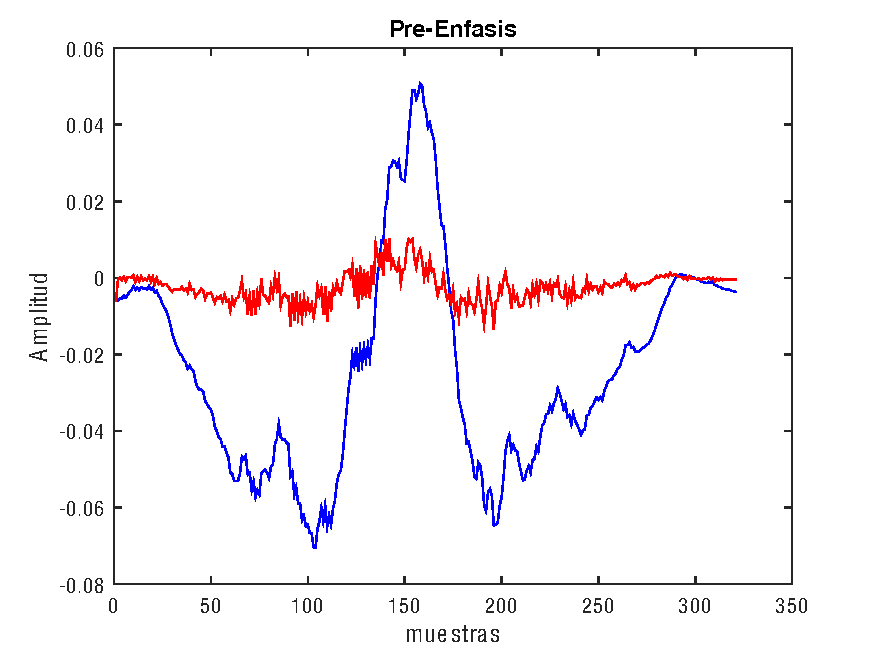
\includegraphics[width=\linewidth]{preenfasis90}
\end{column}
%
\begin{column}{0.5\linewidth}
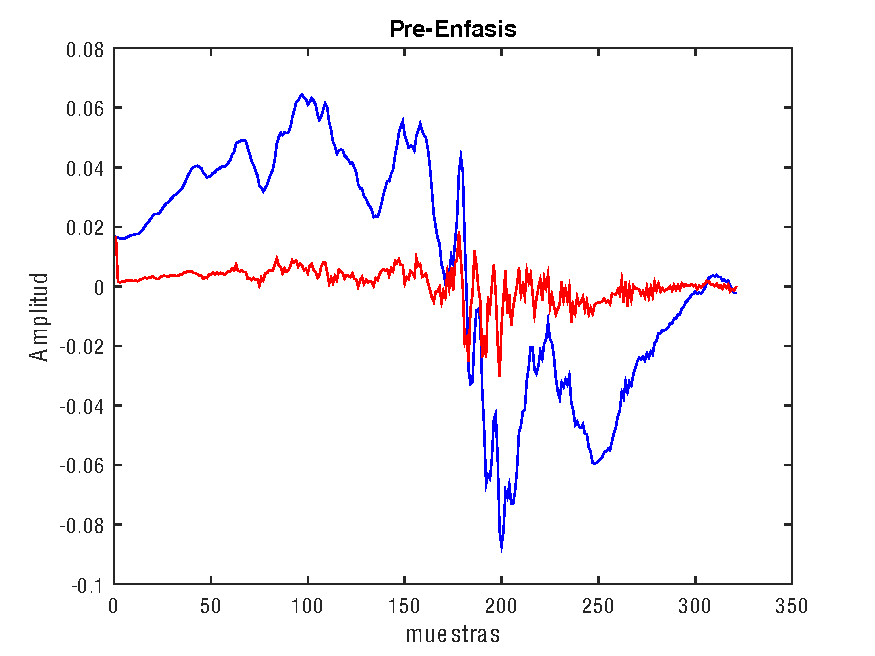
\includegraphics[width=\linewidth]{preenfasis90_1}
\end{column}
\end{columns}

\end{frame}

% 5
\begin{frame}{Frecuencias formantes}

\begin{columns}
\begin{column}{0.5\linewidth}
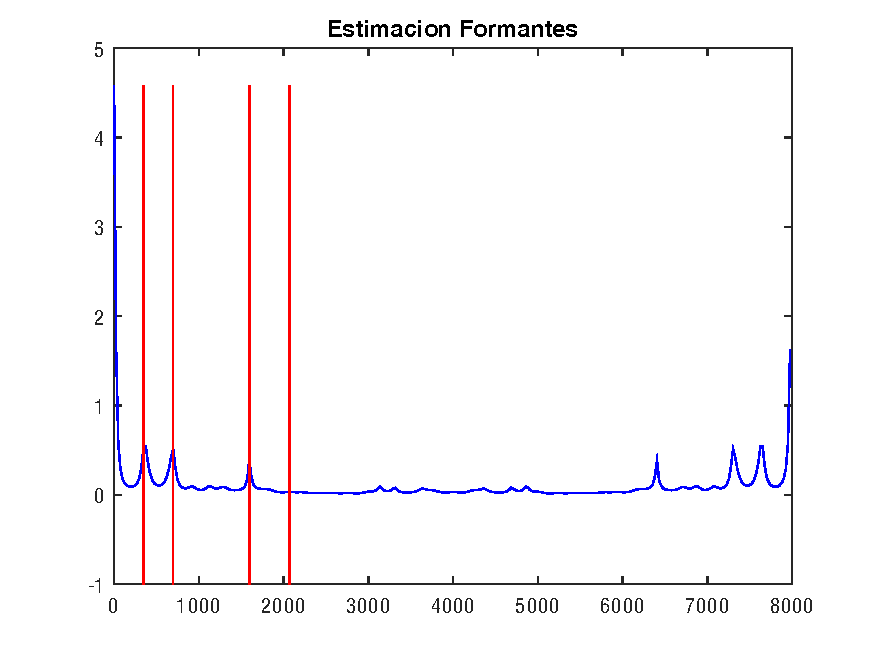
\includegraphics[width=\linewidth]{Formantes} \hfill
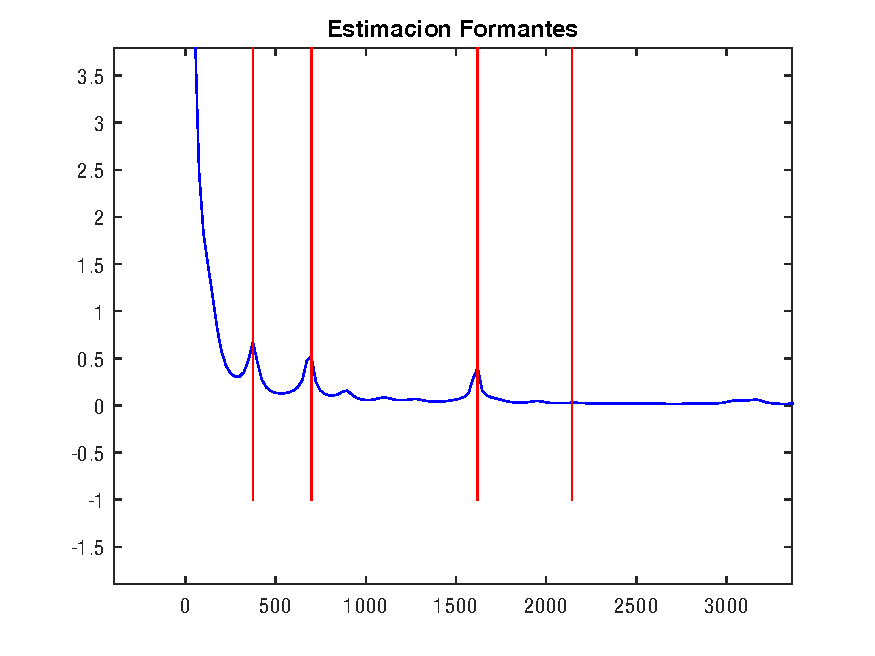
\includegraphics[width=\linewidth]{Formantes2}
\end{column}
%---
\begin{column}{0.5\linewidth}
\begin{enumerate}
\item Respuesta en frecuencia. Predicción lineal. Wiener-Hopf.
\item Parámetros del sistema y factor de ganancia. Levinson-Durbin.
\item $H(z)$. Máximos locales.
\end{enumerate}
\end{column}
\end{columns}

\end{frame}

% 6
\begin{frame}{MFCC}

\begin{enumerate}
\item Ventana. DFT.
\item Filtros triangulares.
\item $\displaystyle F_{mel}=1000\log_{2}\left(1+\frac{F_{Hz}}{1000}\right)$
\item IDFT.
\end{enumerate}

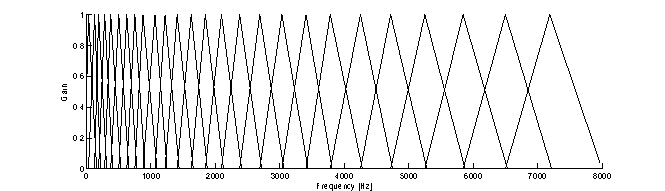
\includegraphics[width=\linewidth]{8}

\end{frame}

% 7
\begin{frame}{DTW}

\begin{columns}
\begin{column}{0.5\linewidth}
\begin{center}
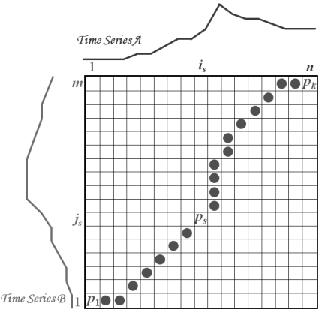
\includegraphics[width=0.7\linewidth]{27}
\end{center}
\end{column}
%---
\begin{column}{0.5\linewidth}
\begin{center}
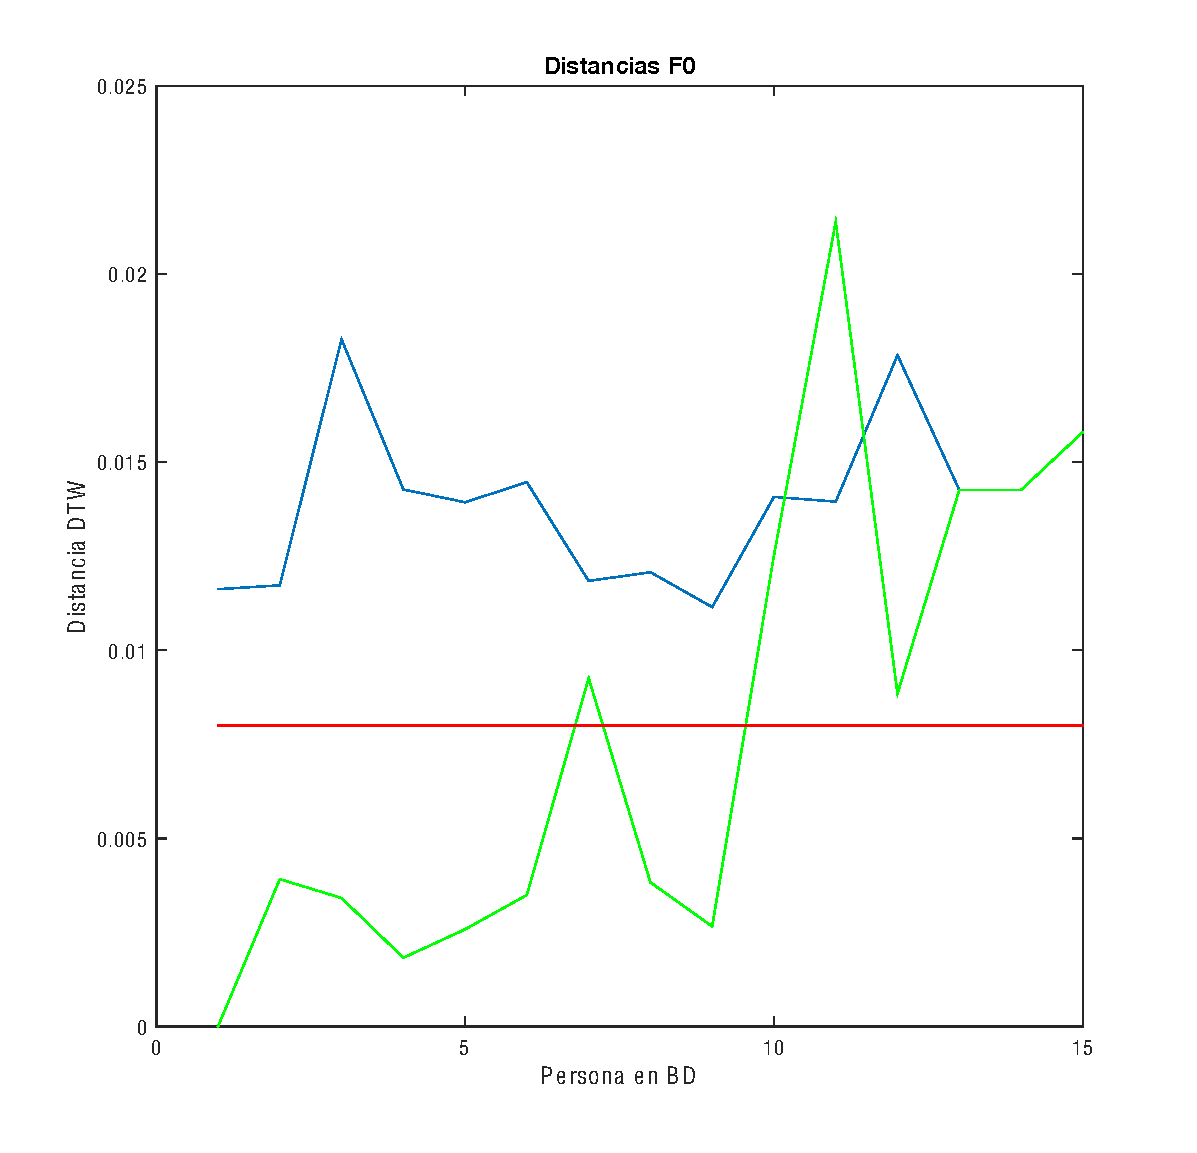
\includegraphics[width=0.7\linewidth]{dF0} \hfill
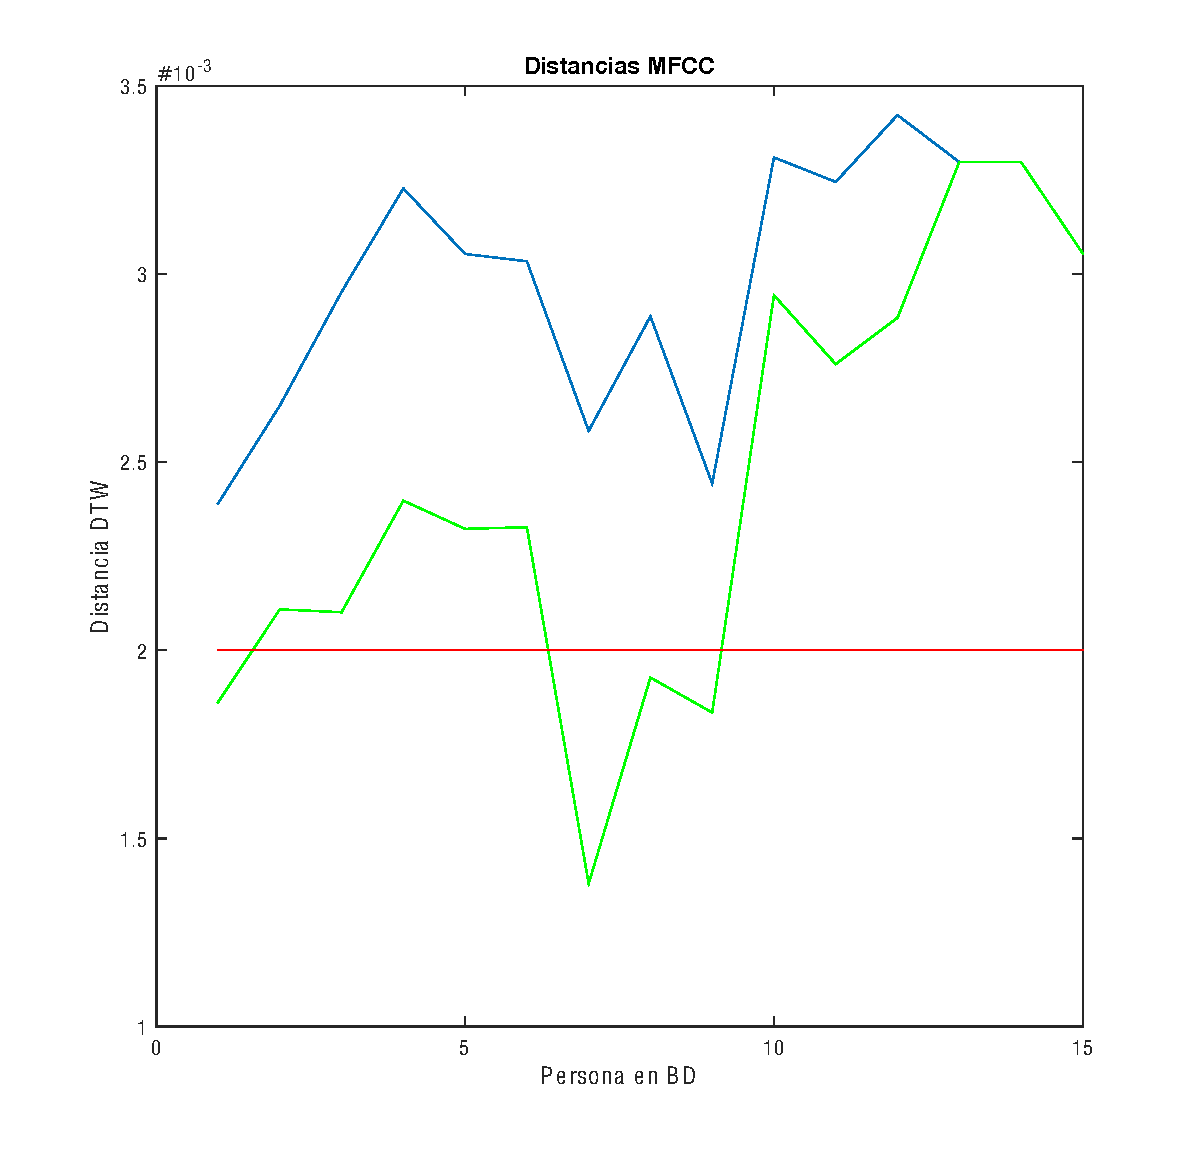
\includegraphics[width=0.7\linewidth]{dMFCC}
\end{center}
\end{column}

\end{columns}

\end{frame}

% 8
\begin{frame}{Resultados}

\begin{center}
\begin{tabular}{cccc} \toprule
Intento / Persona & $F_{0}$ & Formantes & MFCC \\ \midrule
1  & OK    & OK    & OK    \\
2  & OK    & ERROR & OK    \\
3  & OK    & OK    & OK    \\
4  & OK    & ERROR & OK    \\
5  & ERROR & OK    & OK    \\
6  & OK    & OK    & OK    \\
7  & OK    & OK    & OK    \\
8  & OK    & ERROR & OK    \\
9  & ERROR & ERROR & ERROR \\
10 & ERROR & OK    & OK    \\ \bottomrule
\end{tabular}
\end{center}

\end{frame}

\begin{frame}{Resultados}

\begin{center}
DTW - Formantes \\
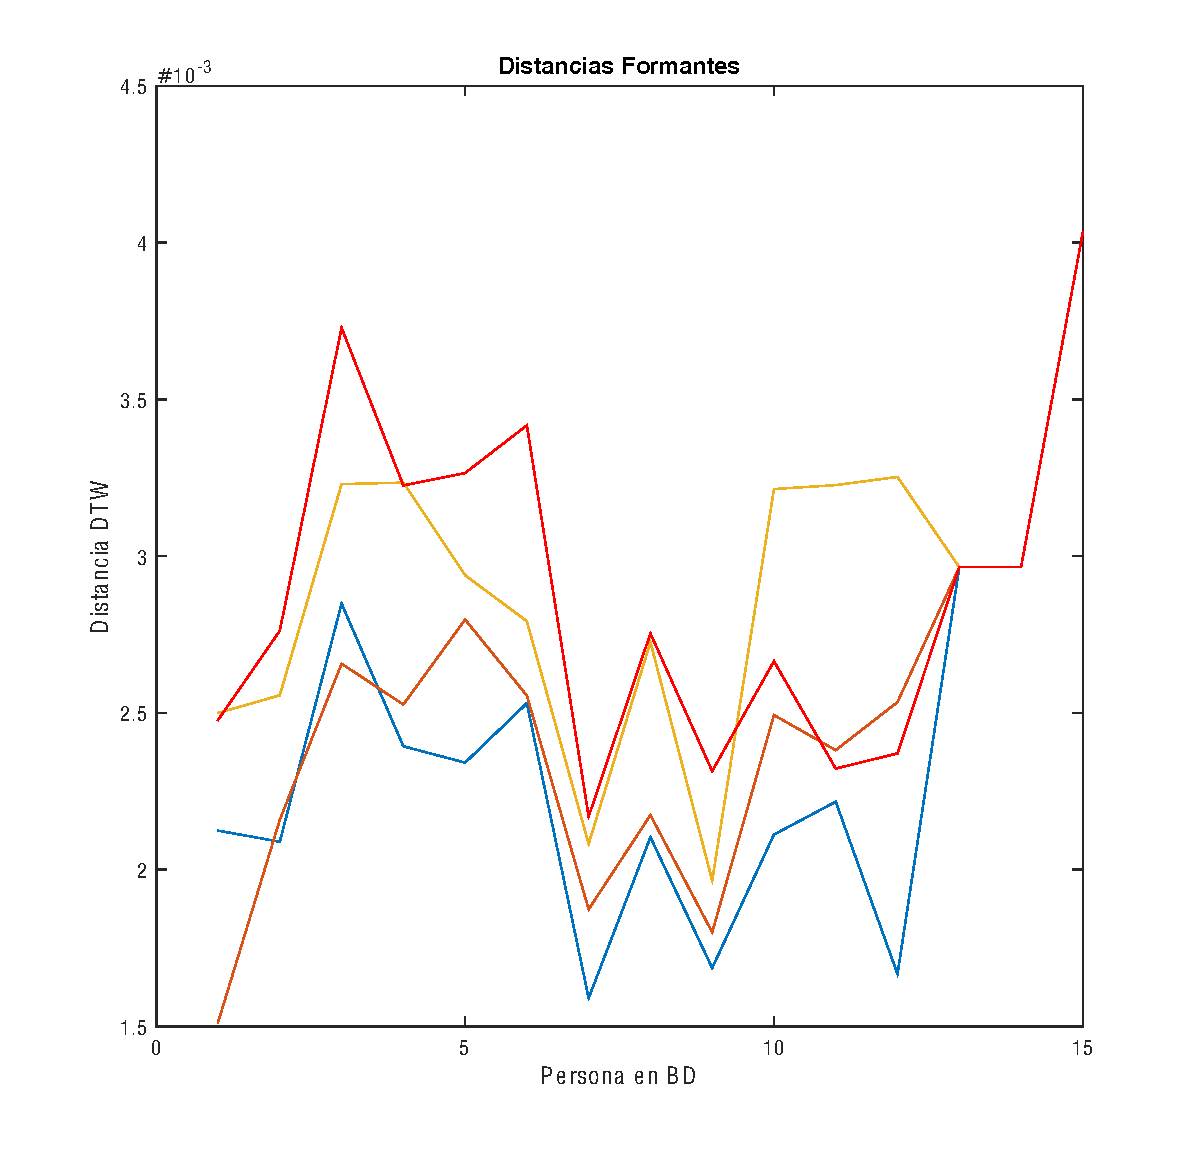
\includegraphics[scale=0.35]{dFor}
\end{center}
\end{frame}

% 9
\begin{frame}{Resultados}

\begin{center}
\begin{tabular}{llcc} \toprule
& & \multicolumn{2}{c}{Valor real} \\
& & V & F \\ \midrule
\multirow{2}{*}{Valor predicto} & V & 8 & 2 \\
& F & 1 & 9 \\ \bottomrule
\end{tabular}
\end{center}

\textit{Sensibilidad:}
$\displaystyle \frac{VP}{(VP+FN)}=\frac{8}{8+2}=0.8$

\textit{Especificidad:}
$\displaystyle \frac{VN}{(VN+FP)}=\frac{9}{9+1}=0.9$

\end{frame}

\begin{frame}{Resultados}

\begin{columns}
\begin{column}{0.6\linewidth}
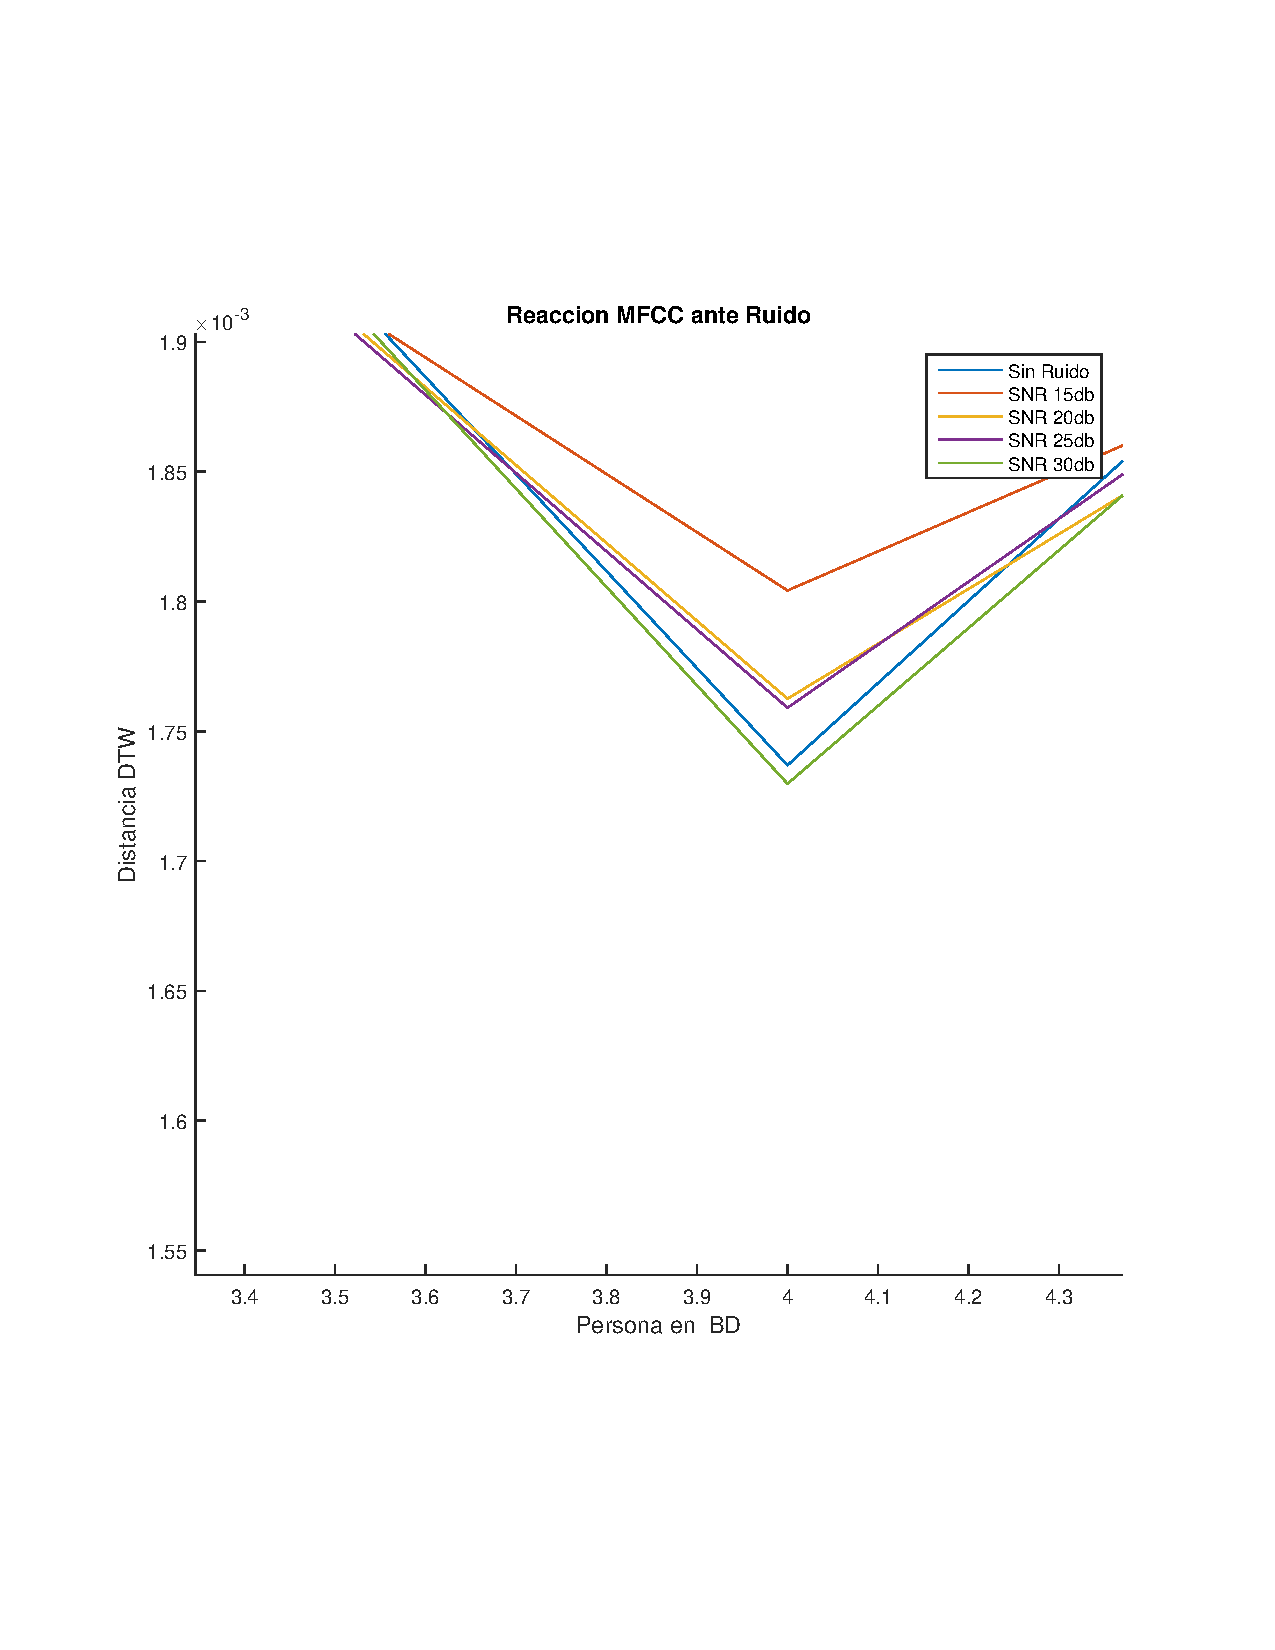
\includegraphics[width=\linewidth]{mfccRuido}
\end{column}

\begin{column}{0.4\linewidth}
Ruido blanco:
 
\begin{quote}
$\mu=0,\sigma=0.5$\\ $SNR = 45[dB]$ \\ 9/10 aciertos.
\end{quote}

Ruido ambiente:

\begin{quote}
$SNR=30[dB]$ \\ 10/10 aciertos \\
$SNR=25[dB]$ \\ 7/10 aciertos
\end{quote}
\end{column}
\end{columns}

\end{frame}

% 10
\begin{frame}{Conclusiones}

\begin{block}{}
\begin{enumerate}
\item $F_{0}$ por si sola no es un buen método de verificación pero complementa.

\item Las \textit{formantes} son poco precisas. Suelen arrojar falsos negativos.

\item Los MFCC son los que arrojan los mejores resultados para la verificación.

\item Todos los métodos son poco robustos al ruido, para que la verificación sea correcta, se necesita una relación señal/ruido de al menos 30 dB.
 
\item Ante la distorsión de la voz de una persona que se encontraba pregrabada en la base de datos, la verificación se muestra inestable.
\end{enumerate}
\end{block}

\end{frame}

% 10
\begin{frame}{Preguntas}


\begin{block}{}
\begin{center}
{\Huge ¿Preguntas?}
\end{center}
\end{block}


\end{frame}
\end{document}